\documentclass[11pt]{article}
\usepackage[utf8]{inputenc}
\usepackage{amsmath, amssymb}
\usepackage{graphicx}
\usepackage{natbib}
\usepackage{geometry}
\usepackage{setspace}
\geometry{margin=1in}
\usepackage{hyperref}
\usepackage{titlesec}
\usepackage{booktabs}
\usepackage{caption}
\usepackage{float}
\usepackage{threeparttable}
\usepackage[english]{babel}


\title{UEFA vs FIFA Tie Break: Which Creates More Suspense?}
\author{Alessandro Di Mattia and Alex Krumer}

\date{}

\begin{document}

\maketitle

\begin{abstract}
This study provides empirical evidence on how tie-breaking rules shape group-level suspense in international football tournaments. By comparing the goal-difference criterion used by FIFA in the World Cup with the head-to-head criterion used by UEFA in the European Championship, we construct a binary suspense indicator that captures whether a single goal could alter the composition of teams qualifying for the knockout stage. Within-group paired tests show that FIFA rules generate significantly higher group-level suspense in the World Cup ($p < 0.01$), while the difference is insignificant in the European Championship. A cross-tournament logit regression controlling for competitive balance finds that World Cup goals are individually less likely to change the qualifying composition — consistent with the FIFA criterion distributing uncertainty more evenly over the group stage rather than concentrating it in a few decisive goals. We further show that suspense under FIFA rules is more stable and persistent over the 90 minutes of play. Together, the evidence points to FIFA's goal-difference criterion as generating more sustained group-level uncertainty in the World Cup.
\end{abstract}

\newpage

\section{Introduction}

In the modern era of sports, and football in particular, retaining audience attention has become both more difficult and more crucial than ever before. Spectators today are exposed to a multitude of entertainment alternatives, making the task of sustaining engagement a key factor for the success and profitability of sport organizations. Beyond loyalty to a specific team, fans gain significant enjoyment from \emph{non-instrumental information}—such as the suspense and uncertainty inherent in a match—which fulfills fundamental psychological needs \citep{ely2015suspense, zillmann2013psychology}. This value often drives consumer interest independently of the game's final result, being rooted instead in the developments that lead to that outcome \citep{vorderer2004enjoyment}.

The economic importance of fan engagement is underscored by the astonishing viewership and revenue generated by major tournaments. For instance, the 2022 FIFA World Cup in Qatar attracted approximately 2.87 billion viewers who watched at least one minute of coverage, while over 5 billion people engaged across broadcast, digital, and social media platforms, including 2.9 billion via linear TV and 2.7 billion through digital streaming \citep{fifa2022engagement, fifa2022audience}. Broadcasting and commercial rights from this World Cup cycle generated over USD 6.3 billion for FIFA, representing 83\% of the organization's revenue \citep{fifa2022finance}.

Similarly, the UEFA European Championship continues to attract massive audiences, with Euro 2024 welcoming a cumulative stadium attendance of 2.67 million across its 51 matches and 5.7 billion viewers worldwide through television \citep{uefa2024numbers, uefa2024remember}. These figures confirm that maintaining audience attention translates directly into financial success.

Given these stakes, the challenge for sports institutions is not only to increase the number of matches, but to design competitions that maximise suspense and engagement. Low-stakes games may decrease overall interest, while mechanisms that preserve uncertainty — such as tie-breaking rules — can extend fan attention across the tournament. Understanding how tie-breaking procedures influence suspense is therefore not only a matter of sporting fairness, but also of monetary relevance, as it directly affects consumer demand, broadcaster revenues, and sponsor value.

In this paper, we investigate how alternative tie-breaking rules influence the level of suspense in international football tournaments. In particular, we compare the two main approaches adopted by governing bodies: FIFA's adoption of overall goal difference and goals scored, and UEFA's use of head-to-head results. We introduce a binary suspense indicator at the group level that captures whether a single goal could alter the composition of teams qualifying for the knockout stage — a concept that is, to the best of our knowledge, new in the sports economics literature. Our main result is that FIFA's goal-difference criterion generates significantly more group-level suspense in the World Cup, and that this advantage is uniform across groups of varying competitive balance. We further document that suspense under FIFA rules is more stable and persistent over the 90 minutes of play. Interestingly, the same advantage does not materialise in the European Championship, where the choice of rule does not significantly affect suspense — a pattern we interpret as a placebo-style robustness check.

\vspace{0.5em}

The structure of the paper is as follows. Section~\ref{sec:literature} reviews the relevant literature. Section~\ref{sec:data} presents the data, while Section~\ref{sec:estimation} outlines the methodological framework. Section~\ref{sec:results} reports the results, and Section~\ref{sec:conclusion} concludes. Additional analyses — including correlation tables, suspense trajectories by group type, and match-level suspense measures — can be found in the Appendix.

\section{Literature Review}
\label{sec:literature}

Our paper lies at the intersection of tournament design and the drivers of sport consumption. Recent contributions in sports economics have highlighted critical flaws in the rules and formats of international football competitions, showing how these deficiencies affect both the fairness of outcomes and the demand for the game. For instance, \citet{csato2025increasing} propose a novel framework to evaluate the cost of stake-less games in which the result no longer influences qualification — for the newly approved 2026 FIFA World Cup format. Similarly, \citet{lapre2023evolution, lapre2022quantifying} demonstrate how FIFA's seeding system has consistently failed to reduce competitive imbalance, thereby significantly lowering some teams' chances of advancing in the competition. As concerns UEFA regulations, \citet{csato2020neither} show how flaws in the qualification rules can create scenarios where teams are incentivized not to win, revealing incentive-compatibility issues in current tournament designs.

To address such structural weaknesses, researchers have advanced a range of solutions, from probabilistic models that improve the predictive accuracy of ranking algorithms \citep{szczecinski2022fifa}, to deterministic optimal scheduling that reduces collusion and stake-less games \citep{chater2021fixing}. Other studies focus on redesigning tournament formats and rules to eliminate misaligned incentives: this includes alternative qualification systems \citep{guajardo2024tournament}, dynamic three-team formats \citep{troyano2023new}, and double-elimination structures \citep{renno2023double}.

\vspace{0.5em}

A related concern arises with the choice of tie-breaking rules, which directly shapes the fairness and stakes of group-stage matches. For example, \citet{berker2014tie} shows that under certain rules, a team's ranking can depend on the outcome of a match in which it does not participate. Similarly, \citet{csato2023avoid} demonstrates that the likelihood of uncompetitive matches — where teams lack incentives to exert full effort — depends strongly on the tie-breaking criteria adopted. Building on this, \citet{csato2026match} show that the shift from goal difference to head-to-head results as the primary tie-breaking criterion in the 2026 FIFA World Cup increases the share of unimportant last-round matches by approximately 5.6 percentage points, as head-to-head rules restrict the set of possible group rankings after the first two rounds and convert offensive-asymmetric matches — where one team must attack to survive — into unimportant ones where teams have little incentive to exert full effort. These findings highlight that poorly designed tie-breakers not only influence match outcomes but also affect the integrity and attractiveness of competitions.

The consequences of these design flaws are not limited to sporting fairness but extend to the economics of sport consumption. Formats and rules that generate collusion opportunities or reduce competitiveness undermine fan interest, diminishing both the entertainment value and commercial revenues of tournaments. Understanding the drivers of demand for both live attendance and broadcast audiences is therefore essential. Several studies identify in-game dynamics as key factors: \citet{buraimo2020unscripted} show that suspense, surprise, and shock — capturing the tension and emotional intensity of matches — contribute to higher demand, particularly at specific moments of play. Likewise, \citet{alavy2010edge} argue that the progression of the game, rather than its final outcome alone, is crucial, with greater uncertainty about results increasing spectator engagement. Similarly, \citet{bizzozero2016importance} find a strong link between suspense and surprise on the one hand, and the demand for entertainment on the other. \citet{flepp2026suspense} further show that the relative importance of suspense and surprise depends on the scoring rate of the match: in high-scoring games, surprise dominates as goals frequently overturn expectations, whereas in low-scoring games sustained suspense becomes the primary driver of engagement. Finally, \citet{buraimo2022armchair} extend this perspective to television audiences, showing that demand cannot be explained solely by uncertainty of outcome but also depends on players' quality and the significance of the match.

Taken together, this domain of research shows that flawed formats and rules do not merely raise ethical and fairness concerns but also undermine the economic value of competitions by reducing engagement and the attractiveness of matches. Our contribution builds on this insight by examining how institutional features — in particular, tie-breaking rules — shape the stakes of a match and, ultimately, its perceived importance in the qualification race. In doing so, we introduce a group-level dimension of suspense that complements the match-level definitions of suspense, surprise, and shock established in the literature: while existing work captures how in-game events shift beliefs about a single match outcome, our measure captures how those same events reshape the broader qualification picture across the group, adding a layer of uncertainty that match-level metrics alone cannot capture.



\section{Data}
\label{sec:data}

This study is based on a detailed dataset of all group stage matches from the FIFA World Cup and UEFA European Championship, focusing on goal-level and minute-by-minute match events. The data were scraped from Wikipedia and cross-checked with official sources from FIFA and UEFA. This allowed us to reconstruct how group standings evolved during matches under each tournament's tie-breaking criteria, enabling a direct comparison of the suspense created by the two systems.

For the FIFA World Cup, we collected data from the 1986 to 2022 editions. From 1986 to 1994, there were 6 groups (Groups A to F), while from 1998 onwards the tournament expanded to 8 groups, each consisting of four teams. In the 6-group format, the top two teams from each group and the four best third-placed teams advanced to the knockout stage, whereas in the 8-group format only the top two teams in each group qualified for the elimination phase. Our dataset includes 455 goals, expanding to 6,789 entries when considering events recorded minute by minute.

For the European Championship, we collected data from 1984 to 2024. The first three editions had two groups (Group 1 and Group 2), then from 1996 to 2012 there were four groups (Groups A to D), and from 2016 onwards six groups (Groups A to F). As in the World Cup, the format with six groups allows the top two teams and the four best third-placed teams to qualify for the next round. In total, we recorded 270 goals and 4,044 minute-by-minute observations.

In both competitions, teams received two points for a win until 1992, and three points from 1994 onwards. One point was awarded for a draw, and zero for a loss throughout all editions.


\subsection{Data Collection}

For every match in both competitions, we collected the following information:

\begin{itemize}
    \item \textbf{Goals scored}: including the scoring team, exact minute, and the evolving scoreline.
    \item \textbf{Team Elo ratings}: Elo ratings as of the day before each tournament began, retrieved from \url{https://www.international-football.net/}.
\end{itemize}

Goal data were used to reconstruct real-time group standings after each event, under both FIFA and UEFA tie-breaking criteria. Elo ratings are used to measure competitive balance at both the group level and the match level, as described in Section~\ref{sec:results}. The minute-by-minute dataset spans from minute 1 to minute 90 for each match, with the exception of matches in which at least one goal was scored in extra time, where observations extend beyond minute 90.


\section{Methodological Framework}
\label{sec:estimation}

Our main contribution is a \textit{binary suspense indicator} defined at the group level that captures whether a single goal could alter the composition of teams qualifying for the knockout stage. More precisely: a suspenseful moment occurs when one additional goal in any ongoing group match would change which teams advance. The indicator is evaluated using two tracking procedures:

\begin{itemize}
    \item \textbf{After each goal scored}, by updating the group standings with the current match results.
    \item \textbf{Minute by minute}, to track the evolution of suspense on a 90-minute scale.
\end{itemize}

This allows us to examine how long a group remains undecided, and how often suspense arises, under the two tie-breaking rules.

For example, in Group F of Euro 2024, entering the third and final matchday, Portugal and Turkey were in qualifying positions for the knockout stage. However, Turkey was playing against Czech Republic, and the match started 0--0. In that situation, a single goal by Czech Republic would have allowed them to overtake Turkey on points and qualify instead. Since the qualification status could change dramatically with just one goal, this scenario is marked as having maximum suspense (suspense~$= 1$).

Another example can be drawn from Group A of Euro 2024. In the final matchday, Hungary scored in the 100th minute against Scotland, winning the match 1--0. At that point, this late goal put Hungary at 3 points with a goal difference of $-3$, making them temporarily one of the best third-placed teams and therefore potentially qualifying for the knockout stage. Suspense is evaluated based on the uncertainty during the match, not on outcomes from matches that are played in later groups, so this goal qualifies as a suspenseful moment at the time it occurs.

A particularly vivid illustration of the \textit{qual\_count} variable is provided by Group~E of the 2022 FIFA World Cup, which included Spain, Germany, Japan, and Costa Rica. Entering the final matchday, Spain and Japan occupied the two qualifying positions; Germany and Costa Rica were eliminated. As both matches — Spain vs.\ Japan and Costa Rica vs.\ Germany — were played simultaneously, the qualifying composition changed four times. Germany's goal at minute~10 moved them above Japan into second place. Japan's equaliser against Spain at minute~48 reclaimed their qualifying spot and sent Germany back out. A Costa Rica goal at minute~70 dramatically reshuffled the standings once more, briefly making Costa Rica and Japan the two qualifiers. A further Costa Rica goal at minute~73 changed the set yet again. By the final whistle, Japan and Spain had qualified, but not before \textit{qual\_count} had reached four — illustrating how the FIFA goal-difference criterion can create repeated and rapid swings in the qualifying composition over the course of simultaneous play.

A full explanation of the logic behind the suspense indicator - covering all specific cases under both FIFA and UEFA rules - is provided in Appendix~\ref{sec:suspense-criteria}.


\section{Results}
\label{sec:results}

\subsection{Descriptive Statistics}

\begin{table}[H]
\centering
\caption{Descriptive statistics -- Goal-level dataset}
\label{tab:desc_stats_goals}
\begin{threeparttable}
\begin{tabular}{lrrrrrrrr}
\toprule
 & \multicolumn{4}{c}{World Cup (FIFA rules)} & \multicolumn{4}{c}{Euro (UEFA rules)} \\
\cmidrule(lr){2-5}\cmidrule(lr){6-9}
 & Mean & SD & Min & Max & Mean & SD & Min & Max \\
\midrule
Goal minute        & 51.99 & 26.89 &  1 &  96 & 52.41 & 26.30 &  2 & 100 \\
Half time          &  1.60 &  0.49 &  1 &   2 &  1.61 &  0.49 &  1 &   2 \\
Qual.\ changed     &  0.19 &  0.39 &  0 &   1 &  0.29 &  0.46 &  0 &   1 \\
Qual.\ count       &  0.72 &  0.99 &  0 &   4 &  1.12 &  1.31 &  0 &   6 \\
Suspense           &  0.44 &  0.50 &  0 &   1 &  0.49 &  0.50 &  0 &   1 \\
Elo (favourite)    & 1904.6 & 106.8 & 1644 & 2169 & 1940.8 &  84.5 & 1671 & 2127 \\
Elo (underdog)     & 1730.4 &  95.3 & 1460 & 1944 & 1812.0 & 102.1 & 1523 & 2040 \\
Elo 1st            & 1987.9 &  77.1 & 1845 & 2169 & 1998.4 &  58.3 & 1850 & 2127 \\
Elo 2nd            & 1855.7 &  63.6 & 1678 & 1986 & 1909.6 &  71.9 & 1766 & 2043 \\
Elo 3rd            & 1777.7 &  61.4 & 1644 & 1920 & 1843.0 &  69.3 & 1671 & 1973 \\
Elo 4th            & 1668.1 &  72.4 & 1460 & 1852 & 1748.6 &  86.0 & 1523 & 1912 \\
\midrule
Observations       & \multicolumn{4}{c}{381} & \multicolumn{4}{c}{226} \\
\bottomrule
\end{tabular}
\begin{tablenotes}
\small
\item \textit{Notes:} Unit of observation is a goal scored on matchday~3. Initial-state rows (minute~$= 0$, one per group per matchday) are excluded. \textit{Qual.\ changed} equals~1 when the set of qualifying teams changes from one goal to the next. \textit{Qual.\ count} is the cumulative number of such changes within the group. \textit{Suspense} equals~1 when the next goal would change the qualifying composition. \textit{Elo (favourite)} and \textit{Elo (underdog)} are the Elo ratings of the stronger and weaker team in each match. \textit{Elo 1st}--\textit{Elo 4th} are group-level Elo ranks from highest to lowest.
\end{tablenotes}
\end{threeparttable}
\end{table}

\begin{table}[H]
\centering
\caption{Descriptive statistics – Minute by Minute events }
\label{tab:desc_stats_mbm}
\begin{tabular}{lrrrrrrrr}
\toprule
\textbf{Variable} & \multicolumn{4}{c}{FIFA rules} & \multicolumn{4}{c}{UEFA rules} \\
 & Mean & St. Dev. & Min & Max & Mean & St. Dev. & Min & Max \\
\midrule
\textbf{Panel A: World Cup} \\
Qualification changed & 0.20  & 0.40  & 0 & 1 & 0.19  & 0.39  & 0 & 1 \\
Qualification count   & 0.63  & 0.87  & 0 & 4 & 0.59  & 0.90  & 0 & 5 \\
Suspense              & 0.45  & 0.50  & 0 & 1 & 0.38  & 0.48  & 0 & 1 \\
Elo home             
& 1789  & 122   & 1492 & 2090 & 1789  & 122   & 1492 & 2090 \\
Elo away              & 1841  & 142   & 1460 & 2169 & 1841  & 142   & 1460 & 2169 \\
\textit{Observations} & \multicolumn{4}{c}{5,204} & \multicolumn{4}{c}{5,204} \\
\midrule
\textbf{Panel B: Euro} \\
Qualification changed & 0.35  & 0.48  & 0 & 1 & 0.33  & 0.47  & 0 & 1 \\
Qualification count   & 1.06  & 1.29  & 0 & 6 & 0.94  & 1.20  & 0 & 6 \\
Suspense              & 0.51  & 0.50  & 0 & 1 & 0.50  & 0.50  & 0 & 1 \\
Elo home              
& 1848  & 113   & 1600 & 2077 & 1848  & 113   & 1600 & 2077 \\
Elo away              & 1880  & 121   & 1523 & 2127 & 1880  & 121   & 1523 & 2127 \\
\textit{Observations} & \multicolumn{4}{c}{2,979} & \multicolumn{4}{c}{2,979} \\
\bottomrule
\end{tabular}
\end{table}


Table~\ref{tab:desc_stats_goals} reports descriptive statistics for the goal-level dataset, comparing World Cup groups (which operate under FIFA tie-breaking rules) with European Championship groups (which operate under UEFA rules). The World Cup sample counts 381 goal events across 74 groups; the European Championship sample counts 226 goal events across 44 groups. Across the key outcome variables, the raw means reveal a consistent pattern: \textit{qual.\ changed} averages 0.19 for the World Cup versus 0.29 for the European Championship, \textit{qual.\ count} averages 0.72 versus 1.12, and \textit{suspense} averages 0.44 versus 0.49. In all three cases, European Championship groups exhibit higher average values than World Cup groups. European Championship teams also tend to be slightly stronger on average: mean Elo ratings for the top-ranked team in each group are 1998 (EU) versus 1988 (WC).

Table~\ref{tab:desc_stats_mbm} reports the same comparison for the minute-by-minute dataset (6{,}789 World Cup and 4{,}044 European Championship match minutes). The pattern is consistent: \textit{qual.\ changed} averages 0.15 (WC) versus 0.24 (EU), \textit{qual.\ count} 0.48 versus 0.69, and \textit{suspense} 0.50 versus 0.57.

\subsection{Statistical Tests}

\begin{table}[H]
\centering
\small
\caption{Differences between UEFA and FIFA tiebreak rules: mean differences and statistical tests}
\label{tab:tests_diff}
\begin{threeparttable}
\begin{tabular}{lcc}
\toprule
\multicolumn{3}{c}{\textbf{European Championship}} \\
\midrule
\textbf{Metric} & Mean Diff. & p-value \\
\midrule
Qualification Count & -0.106 & 0.182 (t-test), 0.250 (Wilcoxon) \\
Suspense            & -0.015 & 0.389 (t-test), 0.438 (Wilcoxon) \\
\midrule
\multicolumn{3}{c}{\textbf{World Cup}} \\
\midrule
\textbf{Metric} & Mean Diff. & p-value \\
\midrule
Qualification Count & -0.024 & 0.535 (t-test), 0.605 (Wilcoxon) \\
Suspense            & -0.040 & 0.008 (t-test), 0.010 (Wilcoxon) \\
\bottomrule
\end{tabular}
\begin{tablenotes}[flushleft]
\small
\textit{Note:} Reported values are mean differences computed as UEFA $-$ FIFA over all groups
(44 European Championship groups; 74 World Cup groups). The paired t-test evaluates
differences in means under approximate normality; the Wilcoxon signed-rank test provides
a non-parametric check. Zero differences are excluded from the Wilcoxon test.
\end{tablenotes}
\end{threeparttable}
\end{table}


Table~\ref{tab:tests_diff} reports paired t-tests and Wilcoxon signed-rank tests comparing group-level mean suspense and mean qualification count across all 74 World Cup groups and all 44 European Championship groups. For the World Cup, the two tie-breaking rules produce markedly different levels of suspense: FIFA rules generate significantly higher group-level suspense than UEFA rules ($p<0.01$, both tests), while the frequency of actual qualification turnover shows no statistically significant difference across the two systems ($p=0.535$). This separation is important: the FIFA rule increases the number of \textit{potential} qualification changes — and hence suspense — without necessarily changing the frequency of \textit{actual} changes in the qualifying composition.

For the European Championship, by contrast, neither suspense nor qualification turnover differs significantly between the two rules ($p=0.389$ and $p=0.182$ respectively). 



\subsection{Suspense over Time}


As shown in Figure~\ref{fig:gls_dist}, the goals distributions for the two competitions appear broadly comparable, with both tournaments showing peaks in goal frequency around the 20th–30th minute in the first half and between the 45th–55th minute spanning the two halves. Toward the end of matches, differences emerge: in the European Championship, there is a distinct peak between the 80th–85th minute, while in the World Cup goals are more evenly spread across the 80th–90th minute. Overall, World Cup goals appear more evenly distributed across the full 100 minutes of play, whereas the European Championship exhibits sharper jumps in specific intervals.

\begin{figure}[H]
    \centering
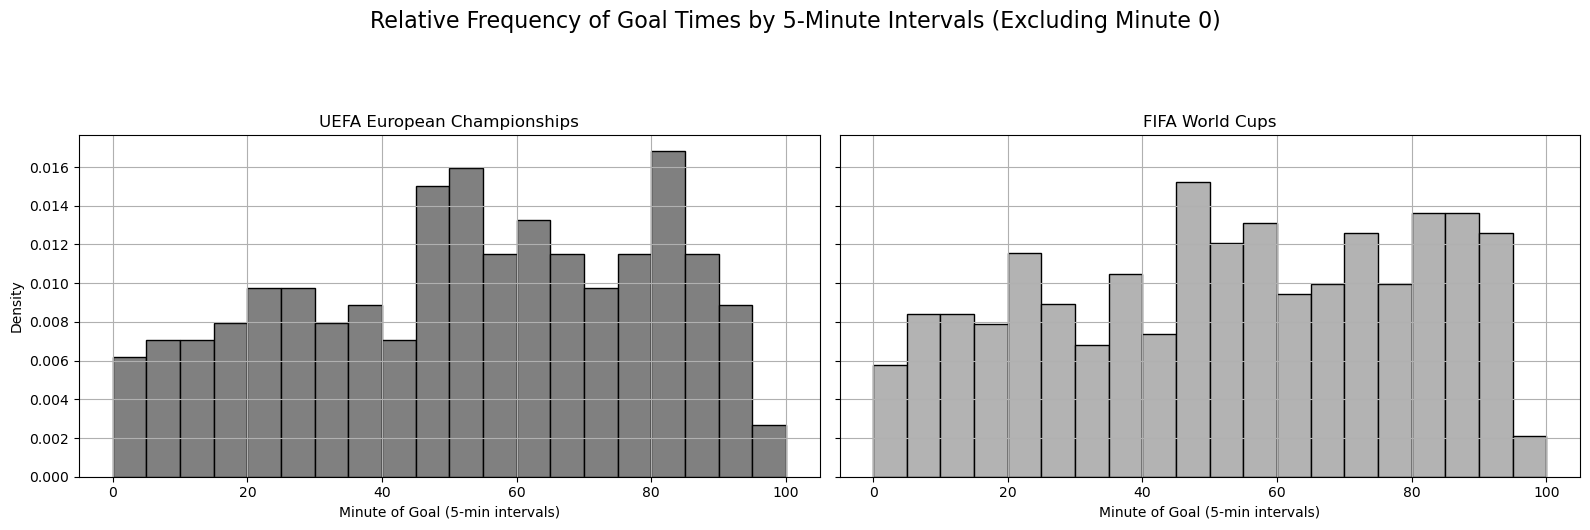
\includegraphics[width=1\textwidth]{images/gls_dist.png}
    \caption{Goals distribution Europe vs World Cup}
    \label{fig:gls_dist}
\end{figure}

Figures~\ref{fig:susp_minute_wc} and~\ref{fig:susp_minute_eu} display the average suspense per minute under each rule for the World Cup and the European Championship respectively. In the World Cup, FIFA rules generate systematically higher suspense across the full 90 minutes, with the gap largest in the final stage of the match. In the European Championship, by contrast, the difference between the two rules is small and — consistent with the statistical tests — not statistically significant. The contrast between the two panels makes the point directly: the effect of the tie-breaking rule on suspense is specific to the World Cup and does not arise  from how the rules operate in any tournament context.

\begin{figure}[H]
    \centering
    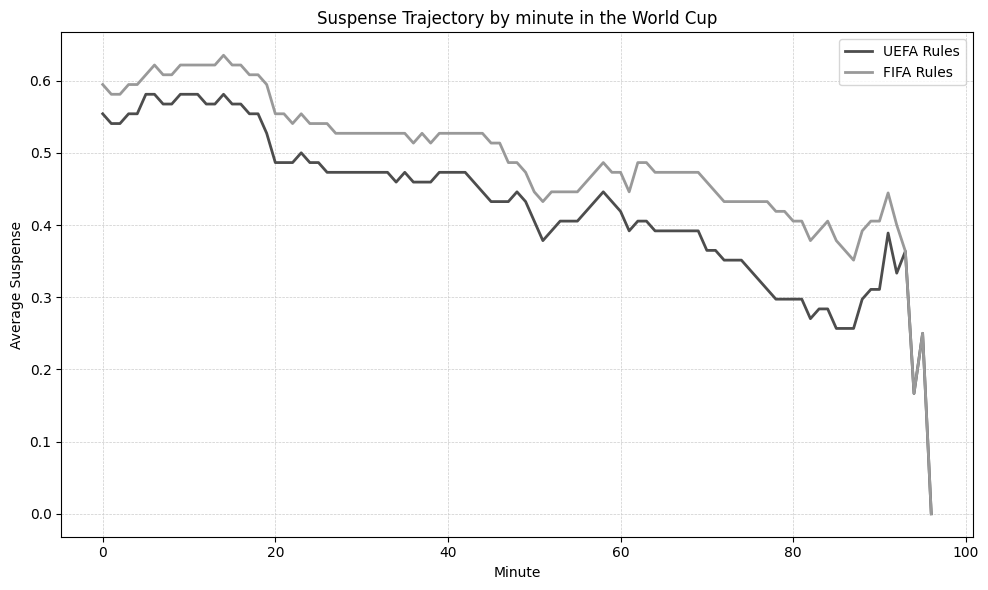
\includegraphics[width=1\textwidth]{images/susp_minute_wc.png}
    \caption{Average suspense per minute under FIFA and UEFA rules — World Cup.}
    \label{fig:susp_minute_wc}
\end{figure}

\begin{figure}[H]
    \centering
    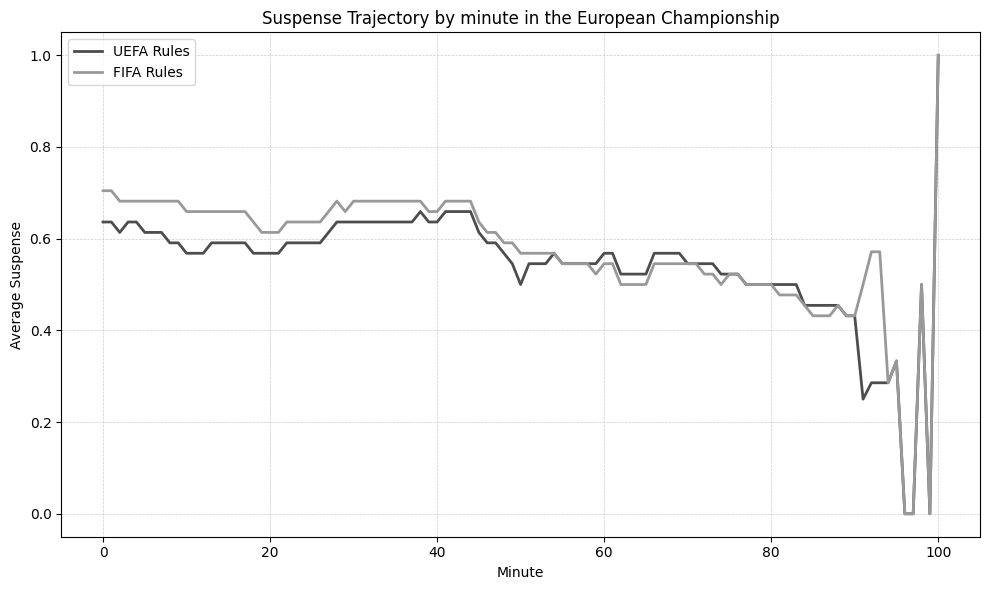
\includegraphics[width=1\textwidth]{images/susp_minute_eu.png}
    \caption{Average suspense per minute under FIFA and UEFA rules — European Championship.}
    \label{fig:susp_minute_eu}
\end{figure}

This pattern is consistent with \citet{csato2023avoid}, who, analysing the 2022/23 UEFA Nations League, argues from a theoretical perspective and through simulated outcomes that prioritising goal difference (FIFA) over head-to-head (UEFA) criteria raises the stakes of matches toward the end of competition. Figure~\ref{fig:susp_minute_wc} provides direct empirical support for this mechanism in the World Cup context. A breakdown of suspense trajectories by group type for both tournaments is reported in Appendix~\ref{app:wc_trajectories} and Appendix~\ref{app:euro_trajectories}.





\subsection{Regression Analysis}

We estimate seven models to test whether the FIFA rule is associated with more frequent qualification changes and higher suspense, after controlling for competitive balance. All logit models report average marginal effects (AME) with standard errors clustered at the group (year~$\times$~stage) level. 

\paragraph{Model 1 — Logit for qualification change, match-level Elo (Table~\ref{tab:reg_grp}).}
The unit of observation is a goal $k$ in group $g$. The dependent variable is \textit{qual\_changed}, a binary indicator equal to~1 when the set of qualifying teams changes from one goal to the next:
\[
\Pr(\textit{qual\_changed}_{gk} = 1)
  = \Lambda\!\left(\alpha + \beta\,\textit{FIFA\_rule}_g
  + \gamma_1\,\textit{elo\_fav}_{gk} + \gamma_2\,\textit{elo\_under}_{gk}\right)
\]
where $\Lambda(\cdot)$ is the logistic CDF, \textit{elo\_fav} and \textit{elo\_under} are the Elo ratings of the stronger and weaker team in the match respectively.

\paragraph{Model 2 — Logit for qualification change, group-level Elo ranks (Table~\ref{tab:reg_grp}).}
The match-level Elo controls are replaced by the four group-level Elo ranks (\textit{elo1st}--\textit{elo4th}, from highest to lowest within the group), which characterise the overall competitive balance of the group rather than the specific match:
\[
\Pr(\textit{qual\_changed}_{gk} = 1)
  = \Lambda\!\left(\alpha + \beta\,\textit{FIFA\_rule}_g
  + \sum_{r=1}^{4} \gamma_r\,\textit{elo}^{(r)}_g\right)
\]

\paragraph{Model 3 — Poisson for qualification count (Table~\ref{tab:reg_grp}).}
The data are collapsed to one observation per group using the maximum value of \textit{qual\_count}, which records the cumulative number of times the qualifying composition changed within a group. A Poisson regression with robust standard errors is estimated:
\[
\mathbb{E}[\textit{qual\_count}_g]
  = \exp\!\left(\alpha + \beta\,\textit{FIFA\_rule}_g
  + \sum_{r=1}^{4} \gamma_r\,\textit{elo}^{(r)}_g\right)
\]

\paragraph{Models 4 \& 5 — Logit for suspense, goal level (Table~\ref{tab:reg_susp}).}
To test whether the FIFA rule is associated with higher suspense at the moment of each goal, we re-estimate the logit framework with \textit{suspense} replacing \textit{qual\_changed} as the dependent variable, using the same goal-level dataset. Model~4 retains match-level Elo controls (\textit{elo\_fav}, \textit{elo\_und}); Model~5 uses group-level Elo ranks (\textit{elo1st}--\textit{elo4th}).

\paragraph{MBM Models — Logit for suspense and qualification change (Table~\ref{tab:reg_mbm}).}
At the minute-by-minute level, we estimate two logit models using group-level Elo controls (\textit{elo1st}--\textit{elo4th}). MBM-A uses the binary \textit{suspense} indicator as the dependent variable. MBM-B uses \textit{qual\_changed}, testing whether the FIFA rule is associated with changes in the qualifying composition at the minute level.


\begin{table}[H]
\centering
\caption{Group-level paired regression: $\Delta\,\overline{\text{suspense}}_g = \overline{\text{suspense}}^{\text{FIFA}}_g - \overline{\text{suspense}}^{\text{UEFA}}_g$}
\label{tab:regression_grp}
\begin{threeparttable}
\begin{tabular}{lcccc}
\toprule
 & \multicolumn{2}{c}{European Championship} & \multicolumn{2}{c}{World Cup} \\
\cmidrule(lr){2-3}\cmidrule(lr){4-5}
 & (1a) & (1b) & (2a) & (2b) \\
\midrule
Elo std & -0.0003 & -0.0001 & -0.0005 & -0.0004 \\
        & (0.0005) & (0.0006) & (0.0003) & (0.0003) \\
\midrule
Year FE & No & Yes & No & Yes \\
N groups & 42 & 42 & 73 & 73 \\
\bottomrule
\end{tabular}
\begin{tablenotes}
\small
\item OLS with HC1 robust standard errors.
Dependent variable is the within-group difference in mean suspense (FIFA minus UEFA).
$^{*}p<0.10$, $^{**}p<0.05$, $^{***}p<0.01$.
\end{tablenotes}
\end{threeparttable}
\end{table}


\begin{table}[H]
\centering
\caption{Effect of FIFA tie-breaking rule on suspense — goal-level logit (AME)}
\label{tab:reg_susp}
\begin{threeparttable}
\small
\begin{tabular}{l cc cc}
\toprule
 & \multicolumn{2}{c}{M4: Match-level Elo} & \multicolumn{2}{c}{M5: Group-level Elo} \\
\cmidrule(lr){2-3}\cmidrule(lr){4-5}
 & (1) Main & (2) $+$Year & (3) Main & (4) $+$Year \\
\midrule
\multicolumn{5}{l}{\textit{Panel A: Main specifications}} \\[2pt]
FIFA\_rule & $-0.015$ & $-0.001$ & $\phantom{-}0.019$ & $\phantom{-}0.044$ \\
          & $(0.075)$ & $(0.077)$ & $(0.075)$ & $(0.076)$ \\[3pt]
Match-level Elo (\textit{elo\_fav}, \textit{elo\_und}) & \checkmark & \checkmark & -- & -- \\
Group-level Elo (\textit{elo1st}--\textit{elo4th})    & -- & -- & \checkmark & \checkmark \\
Year trend & -- & \checkmark & -- & \checkmark \\[3pt]
Observations & 607 & 607 & 725 & 725 \\
\midrule
\multicolumn{5}{l}{\textit{Panel B: Robustness — FIFA\_rule only (all specifications include year trend)}} \\[2pt]
 & \multicolumn{2}{c}{M4} & \multicolumn{2}{c}{M5} \\
\cmidrule(lr){2-3}\cmidrule(lr){4-5}
Two qualifying teams    & \multicolumn{2}{c}{$-0.080$} & \multicolumn{2}{c}{$-0.036$} \\
                        & \multicolumn{2}{c}{$(0.084)$} & \multicolumn{2}{c}{$(0.090)$} \\
Three qualifying teams  & \multicolumn{2}{c}{$-0.006$} & \multicolumn{2}{c}{$-0.734$} \\
                        & \multicolumn{2}{c}{$(0.642)$} & \multicolumn{2}{c}{$(0.630)$} \\
2-points rule ($\le 1992$) & \multicolumn{2}{c}{$-0.151$} & \multicolumn{2}{c}{$\phantom{-}0.079$} \\
                        & \multicolumn{2}{c}{$(0.160)$} & \multicolumn{2}{c}{$(0.314)$} \\
3-points rule ($> 1992$) & \multicolumn{2}{c}{$\phantom{-}0.031$} & \multicolumn{2}{c}{$\phantom{-}0.068$} \\
                        & \multicolumn{2}{c}{$(0.082)$} & \multicolumn{2}{c}{$(0.080)$} \\
Elo common support      & \multicolumn{2}{c}{$\phantom{-}0.006$} & \multicolumn{2}{c}{$\phantom{-}0.029$} \\
                        & \multicolumn{2}{c}{$(0.080)$} & \multicolumn{2}{c}{$(0.077)$} \\
\bottomrule
\end{tabular}
\begin{tablenotes}
\small
\item \textit{Notes:} Logit model for the binary \textit{suspense} indicator estimated on the goal-level dataset. Coefficients are average marginal effects (AME). M4 controls for match-level Elo ratings (\textit{elo\_fav}, \textit{elo\_und}); M5 uses group-level Elo ranks (\textit{elo1st}--\textit{elo4th}). Standard errors are clustered at the group (year~$\times$~stage) level. Panel~B robustness samples follow the same definitions as in Table~\ref{tab:reg_grp}; all Panel~B specifications include \textit{year\_c}. $^{*}p<0.10$, $^{**}p<0.05$, $^{***}p<0.01$.
\end{tablenotes}
\end{threeparttable}
\end{table}


\begin{table}[H]
\centering
\caption{MBM logit models: effect of FIFA tie-breaking rule on suspense and qualification change}
\label{tab:reg_mbm}
\begin{threeparttable}
\small
\begin{tabular}{l cc cc}
\toprule
 & \multicolumn{2}{c}{MBM-A: \textit{suspense}} & \multicolumn{2}{c}{MBM-B: \textit{qual\_changed}} \\
\cmidrule(lr){2-3}\cmidrule(lr){4-5}
 & (1) Main & (2) $+$Year & (3) Main & (4) $+$Year \\
\midrule
\multicolumn{5}{l}{\textit{Panel A: Main specifications}} \\[2pt]
FIFA\_rule & $-0.031$ & $\phantom{-}0.001$ & $-0.103^{**}$ & $-0.086^{*}$ \\
          & $(0.081)$ & $(0.083)$ & $(0.049)$ & $(0.045)$ \\[3pt]
Group-level Elo controls & \checkmark & \checkmark & \checkmark & \checkmark \\
Year trend (\textit{year\_c}) & -- & \checkmark & -- & \checkmark \\[3pt]
Observations & 10{,}833 & 10{,}833 & 10{,}833 & 10{,}833 \\
Pseudo-$R^2$ & 0.029 & 0.037 & 0.023 & 0.027 \\
\midrule
\multicolumn{5}{l}{\textit{Panel B: Robustness — FIFA\_rule only (all specifications include year\_c)}} \\[2pt]
 & \multicolumn{2}{c}{MBM-A} & \multicolumn{2}{c}{MBM-B} \\
\cmidrule(lr){2-3}\cmidrule(lr){4-5}
Two qualifying teams    & \multicolumn{2}{c}{$-0.084$} & \multicolumn{2}{c}{$-0.049$} \\
                        & \multicolumn{2}{c}{$(0.095)$} & \multicolumn{2}{c}{$(0.052)$} \\
Three qualifying teams  & \multicolumn{2}{c}{$-0.219$} & \multicolumn{2}{c}{$-0.073$} \\
                        & \multicolumn{2}{c}{$(0.753)$} & \multicolumn{2}{c}{$(0.525)$} \\
2-points rule ($\le 1992$) & \multicolumn{2}{c}{$\phantom{-}0.265$} & \multicolumn{2}{c}{$\phantom{-}0.290^{**}$} \\
                        & \multicolumn{2}{c}{$(0.278)$} & \multicolumn{2}{c}{$(0.142)$} \\
3-points rule ($> 1992$) & \multicolumn{2}{c}{$\phantom{-}0.014$} & \multicolumn{2}{c}{$-0.105^{**}$} \\
                        & \multicolumn{2}{c}{$(0.086)$} & \multicolumn{2}{c}{$(0.046)$} \\
Elo common support      & \multicolumn{2}{c}{$-0.012$} & \multicolumn{2}{c}{$-0.083^{*}$} \\
                        & \multicolumn{2}{c}{$(0.084)$} & \multicolumn{2}{c}{$(0.048)$} \\
\bottomrule
\end{tabular}
\begin{tablenotes}
\small
\item \textit{Notes:} Logit models estimated on the minute-by-minute (MBM) dataset. MBM-A uses the binary \textit{suspense} indicator as the dependent variable; MBM-B uses \textit{qual\_changed}, a binary indicator equal to~1 when the qualifying composition changes at that minute. Group-level Elo ranks (\textit{elo1st}--\textit{elo4th}) are included as controls in all specifications. Standard errors are clustered at the group (year~$\times$~stage) level. Panel~B robustness samples follow the same definitions as in Table~\ref{tab:reg_grp}. $^{*}p<0.10$, $^{**}p<0.05$, $^{***}p<0.01$.
\end{tablenotes}
\end{threeparttable}
\end{table}


Table~\ref{tab:reg_grp} reports the estimates for Models~1--3. The coefficient on \textit{FIFA\_rule} is consistently negative across all specifications: World Cup goals are on average 9.7 percentage points less likely to change the qualifying composition than European Championship goals (Model~1, $p = 0.045$, $N = 607$), with a consistent direction in Model~2 ($-6.5$ pp, $p = 0.146$, $N = 725$) and in the Poisson for qualification count (Model~3, coefficient $-0.33$, $p = 0.173$). MBM-B in Table~\ref{tab:reg_mbm} confirms this pattern at the minute level: World Cup minutes are 10.3 percentage points less likely to involve a change in the qualifying composition ($p = 0.034$), with consistent results under the 3-points rule ($-0.105$, $p = 0.021$) and the Elo common support sample ($-0.083$, $p = 0.082$).

The picture is considerably different when the dependent variable is \textit{suspense} — the indicator that the current state is such that one more goal \textit{would} potentially change the qualifying composition. Table~\ref{tab:reg_susp} shows that the FIFA\_rule coefficient in Models~4--5 is small, inconsistent in sign, and never approaches significance ($-0.015$, $p = 0.846$ in Model~4; $+0.019$, $p = 0.800$ in Model~5). MBM-A tells the same story ($-0.031$, $p = 0.696$). The FIFA rule thus reduces the frequency of \textit{actual} changes in the qualifying composition without systematically altering the share of moments that potentially can lead to a change — a distinction between realised turnover and anticipated volatility.

A notable twist emerges from the 2-points versus 3-points rule subsamples. Under the old 2-points system (years $\le 1992$), the FIFA rule is associated with \textit{more} changes in the qualifying composition: $+0.290$ in MBM-B ($p = 0.041$) and a positive but imprecise direction in Models~1--3. Under the modern 3-points system (years $> 1992$), the sign reverses to negative across all models ($-0.105$ in MBM-B, $p = 0.021$). This flip is consistent with the idea that under the old system, the greater prevalence of draws made goal difference a more frequently decisive tiebreaker, so FIFA-rule groups experienced more volatility in the composition of qualifying teams. Once wins became more valuable and draws rarer under the 3-points system, qualification was settled more directly through points, reducing the marginal importance of goal difference and changing the compositional twist that the FIFA rule previously induced. Robustness checks are reported in the same tables.


\section{Conclusion}
\label{sec:conclusion}

This paper was motivated by the question of how alternative tie-breaking criteria shape the level of suspense in international football tournaments. Tie-breaking rules are not merely technical details: they influence the perceived attractiveness of games, with potential implications for revenues, stadium attendance, and viewership. By choosing one criterion over another, governing bodies implicitly decide how much uncertainty to preserve throughout the group stage.

We compared the two main approaches in international football: the FIFA rule, which prioritises goal difference, and the UEFA rule, which prioritises head-to-head results. Our analysis combines two complementary perspectives. Within-group paired tests establish that applying FIFA rules to the same group generates significantly more suspense than the UEFA criterion in the World Cup ($p < 0.01$), while the difference is insignificant in the European Championship. A cross-tournament regression controlling for competitive balance reveals another clear picture: World Cup goals are individually less likely to change the qualifying composition than European Championship goals, suggesting that the FIFA criterion distributes qualification uncertainty more evenly over the course of a group — keeping more scenarios open at any given moment — rather than concentrating it in a smaller number of pivotal goals.

The European Championship serves as an informative contrast: neither the within-group tests nor the cross-tournament regression finds a statistically significant difference in suspense between the two rules. This null result underscores that the effect documented for the World Cup is specific to that competition and does not arise simply from how either rule operates in the abstract.

Overall, our results establish that institutional design choices — specifically, the choice of tie-breaking criterion — have measurable consequences for the suspense experienced by the billions of fans who follow the World Cup. A rule that keeps more qualification scenarios alive for longer raises the entertainment value of each match. Our evidence points to FIFA's goal-difference criterion as generating more sustained group-level uncertainty, a finding with direct relevance for governing bodies as they continue to revise tournament formats and seek to maximise the commercial and sporting value of their competitions.


\bibliographystyle{apalike}
\bibliography{reference}


% ===========================================================================
\appendix
\section*{Appendix}
% ===========================================================================

\subsection{Suspense Criteria: Full Logic}
\label{sec:suspense-criteria}

The following rules describe the exact criteria we use to assign a suspense value of 1 (suspenseful moment) in both FIFA and UEFA group stages. A suspenseful moment is defined as one where a single goal may change the composition of teams qualifying for the knockout stage. These rules are applied after each goal and at each match minute during the group stage.

\subsubsection*{Suspense Criteria: FIFA}
\label{sec:suspense-fifa-implemented}

FIFA ranking within the group follows the tie-break hierarchy:
\[
\text{Points} \;\; \rightarrow \;\; \text{Overall Goal Difference} \;\; \rightarrow \;\; \text{Overall Goals Scored} \;\; \rightarrow \;\; \text{Head-to-Head (if required)}.
\]
We evaluate suspense after each goal/minute observation using the pipeline below.

\paragraph{Step 0: Identify the cut-off pair (leading vs lagging).}
Let \texttt{third\_qualify} indicate whether the relevant cut-off is:
\begin{itemize}
    \item \texttt{third\_qualify = 0}: \textbf{2nd} (leading, last qualified) vs \textbf{3rd} (lagging, first not qualified),
    \item \texttt{third\_qualify = 1}: \textbf{3rd} (leading) vs \textbf{4th} (lagging).
\end{itemize}
We denote the lagging and leading teams' current \emph{overall} differences by:
\[
\texttt{pts\_diff}_0,\;\texttt{gls\_diff}_0,\;\texttt{gs\_diff}_0,
\]
where \texttt{gs\_diff} is computed as goals scored by lagging minus goals scored by leading.

\paragraph{Step 1: Infer current match points from match goal difference.}
At every minute, each team has a match-specific goal difference (\texttt{last\_game\_goals\_diff}).
We infer match points robustly from this match GD:
\[
\texttt{match\_pts} =
\begin{cases}
\texttt{win\_pts} & \text{if match GD} > 0,\\
1 & \text{if match GD} = 0,\\
0 & \text{if match GD} < 0,
\end{cases}
\]
with \texttt{win\_pts} $=2$ if \texttt{year $\le$ 1992} and \texttt{win\_pts} $=3$ otherwise.

\paragraph{Step 2: Evaluate the two one-goal shocks }
% function calculate\_suspense.

We compute whether \emph{either} of the following shocks makes lagging rank $\ge$ leading under FIFA ordering:
\begin{enumerate}
    \item \textbf{Lagging scores (+1)}.
    \item \textbf{Leading concedes (+1)}.
\end{enumerate}

\noindent The shocks update \emph{both} (i) match states and (ii) overall differences:
\begin{itemize}
    \item If \texttt{h2h = 0} (teams are in different matches), the shock affects only the relevant team's match GD by $\pm 1$ and hence may change match points. Overall GD changes by $+1$ in favor of lagging for either shock. Goals scored changes by $+1$ \emph{only} if lagging scores.
    \item If \texttt{h2h = 1} (teams are facing each other in the current match), a single goal simultaneously improves lagging's match GD by $+1$ and worsens leading's match GD by $-1$. Hence overall GD changes by $+2$ in favor of lagging. Goals scored of lagging increases by $+1$.
\end{itemize}

\noindent After updating points (through inferred match points), overall GD, and overall goals scored, suspense is set to 1 if lagging becomes \emph{not behind} leading under:
\[
\text{Points} \rightarrow \text{Overall GD} \rightarrow \text{Overall GS}.
\]
If the shock produces a full tie on all three dimensions, we still classify the moment as suspenseful (\texttt{suspense=1}), since the next tie-break (e.g., head-to-head or lots) may decide qualification.

\paragraph{Step 3: Flag head-to-head tie-break cases }
% function update\_suspense
We create the indicator \texttt{h2h\_suspense} to identify the subset of observations where the qualification cut-off would be decided by the \emph{head-to-head} tie-break between the lagging and leading teams.
Practically, we flag \texttt{h2h\_suspense=1} when a full tie on the \emph{FIFA pre-H2H criteria} (points, overall goal difference, and overall goals scored) can be reached with a single-goal shock from \emph{both} perspectives:
\begin{itemize}
    \item full tie after \textbf{lagging scores (+1)}, and
    \item full tie after \textbf{leading concedes (+1)}.
\end{itemize}
Only for these cases we set \texttt{suspense=1} and \texttt{h2h\_suspense=1}.
This ``both perspectives'' requirement excludes situations where only one shock produces a full tie, while the other shock would already give one team a strict advantage on goals scored.

\paragraph{Step 4: Evaluate the relevant head-to-head match}

% function \texttt{evaluate\_lagging\_losses\_and\_update\_suspense}.

For observations with \texttt{h2h\_suspense=1}, we evaluate the head-to-head status between the lagging and leading teams to determine whether the tie-break can actually favor the lagging team.
There are two distinct cases:
\begin{itemize}
    \item \textbf{\texttt{h2h = 1} (current match):} lagging and leading are facing each other in the ongoing match. In this case, the head-to-head outcome is determined by the \emph{current score} at minute $t$ (i.e., the current match goal difference for the lagging team).
    \item \textbf{\texttt{h2h = 0} (previous match):} lagging and leading are not playing each other in the current match minute; their head-to-head match is in one of the two \emph{previous} fixtures in the same group stage. In this case the head-to-head outcome is fixed and can be retrieved from \texttt{goals\_df} using the match's final score. If the lagging team loses the head-to-head match, we set \texttt{suspense} back to 0 for that observation.
\end{itemize}

\paragraph{Step 5: Draw-lots adjustments.}

% function \texttt{update\_suspense\_draw\_lots}
Finally, we manually set \texttt{suspense=1} in a small set of edge cases where the FIFA rules imply qualification may be decided by lots.

\paragraph{Diagnostic audit: outside-team threat when \texttt{suspense=0}}
% function (\texttt{audit\_suspense0\_where\_4th\_threatens\_2nd\_fifa}).
Because the main suspense logic evaluates only the cut-off pair (leading vs lagging), we also run a diagnostic check for cases with \texttt{suspense=0} and \texttt{third\_qualify=0} where the \textbf{4th} team can reach or overtake the \textbf{2nd} team with one goal shock under FIFA ordering.


\subsubsection*{Suspense Criteria: UEFA}
\label{sec:suspense-uefa-implemented}

For competitions governed by UEFA rules, team ranking within a group follows a different tie-breaking hierarchy:
\begin{enumerate}
    \item total points,
    \item head-to-head result between the tied teams,
    \item overall goal difference,
    \item overall goals scored.
\end{enumerate}
Unlike the FIFA procedure, head-to-head is applied \emph{before} overall goal difference and goals scored.

\paragraph{Step 1: Identify the relevant ranking pair.}
At each observation (defined by a goal minute within a group-stage match), we identify the pair of teams defining the qualification cut-off. When only the top two teams qualify (\texttt{third\_qualify = 0}), the relevant comparison is between the teams ranked second and third. When the third-placed team may also qualify (\texttt{third\_qualify = 1}), the relevant comparison is between the teams ranked third and fourth.

\paragraph{Step 2: Evaluate one-goal shocks.}
For each observation we evaluate whether a single-goal shock could allow the lagging team to reach or overtake the leading team. Two possible shocks are considered: lagging scores one goal (+1) or leading concedes one goal (+1). Match points are inferred from the match goal difference using the appropriate points system.

\paragraph{Step 3: Apply UEFA tie-breaking rules.}
After applying the hypothetical shock, we compare the lagging and leading teams according to the UEFA ranking hierarchy: total points, then head-to-head, then overall goal difference, then overall goals scored. When the two teams are not currently facing each other, the head-to-head outcome is fixed from the previous fixture; when they are playing each other, the current score determines the head-to-head outcome.

\paragraph{Step 4: Determine suspense.}
If under either shock the lagging team becomes at least as well ranked as the leading team, we set \texttt{suspense = 1}.

\paragraph{Step 5: Identify outside-team threats.}
Finally, we check whether the fourth-placed team could reach or overtake the second-placed team with a single-goal shock, applying the full UEFA hierarchy. Observations satisfying this condition are edited separately.


\subsection{Correlation Analysis}
\label{app:correlations}

Tables~\ref{tab:corr_eu}--\ref{tab:corr_wc_mbm} report pairwise correlations between suspense, qualification turnover, and group-level competitive balance (Elo standard deviation) for both tournaments and both datasets.

For the European Championship (Tables~\ref{tab:corr_eu} and~\ref{tab:corr_eu_mbm}), the number of changes in the qualifying composition is positively associated with aggregate suspense in every specification, with the association stronger under FIFA rules. Regarding group imbalance, suspense increases with imbalance under both rules, while the relationship between imbalance and qualification turnover is weak and slightly negative. This is not surprising: qualification turnover captures only actual changes, whereas our suspense measure also accounts for potential changes.

\begin{table}[H]
\centering
\small
\caption{Correlation matrices for goals-based aggregation in UEFA European Championship}
\label{tab:corr_eu}
\begin{tabular}{lccc}
\toprule
 & Elo std & Avg. qual. count & Avg. suspense \\
\midrule
\multicolumn{4}{l}{\textbf{UEFA}} \\
Elo std             & 1.000 & -0.089 & 0.251 \\
Avg. qual. count    & -0.089 & 1.000 & 0.391 \\
Avg. suspense       & 0.251 & 0.391 & 1.000 \\
\midrule
\multicolumn{4}{l}{\textbf{FIFA}} \\
Elo std             & 1.000 & -0.061 & 0.264 \\
Avg. qual. count    & -0.061 & 1.000 & 0.406 \\
Avg. suspense       & 0.264 & 0.406 & 1.000 \\
\bottomrule
\end{tabular}
\end{table}

\begin{table}[H]
\centering
\small
\caption{Correlation matrices for minute-by-minute aggregation in UEFA European Championship}
\label{tab:corr_eu_mbm}
\begin{tabular}{lccc}
\toprule
 & Elo std & Avg. qual. count & Avg. suspense \\
\midrule
\multicolumn{4}{l}{\textbf{UEFA}} \\
Elo std             & 1.000 & -0.102 & 0.175 \\
Avg. qual. count    & -0.102 & 1.000 & 0.299 \\
Avg. suspense       & 0.175 & 0.299 & 1.000 \\
\midrule
\multicolumn{4}{l}{\textbf{FIFA}} \\
Elo std             & 1.000 & -0.036 & 0.153 \\
Avg. qual. count    & -0.036 & 1.000 & 0.351 \\
Avg. suspense       & 0.153 & 0.351 & 1.000 \\
\bottomrule
\end{tabular}
\end{table}


For the World Cup (Tables~\ref{tab:corr_wc} and~\ref{tab:corr_wc_mbm}), the number of changes in the qualifying composition is positively associated with aggregate suspense (correlations around 0.43--0.56), and slightly stronger under FIFA rules. In contrast to the European Championship, suspense is negatively related to group imbalance, indicating that more balanced groups tend to generate higher suspense.

\begin{table}[H]
\centering
\small
\caption{Correlation matrices for goals-based aggregation in FIFA World Cup}
\label{tab:corr_wc}
\begin{tabular}{lccc}
\toprule
 & Elo std & Avg. qual. count & Avg. suspense \\
\midrule
\multicolumn{4}{l}{\textbf{UEFA rule}} \\
Elo std             & 1.000 & -0.064 & -0.184 \\
Avg. qual. count    & -0.064 & 1.000 & 0.456 \\
Avg. suspense       & -0.184 & 0.456 & 1.000 \\
\midrule
\multicolumn{4}{l}{\textbf{FIFA rule}} \\
Elo std             & 1.000 & -0.060 & -0.278 \\
Avg. qual. count    & -0.060 & 1.000 & 0.588 \\
Avg. suspense       & -0.278 & 0.588 & 1.000 \\
\bottomrule
\end{tabular}
\end{table}

\begin{table}[H]
\centering
\small
\caption{Correlation matrices for minute-by-minute aggregation in FIFA World Cup}
\label{tab:corr_wc_mbm}
\begin{tabular}{lccc}
\toprule
 & Elo std & Avg. qual. count & Avg. suspense \\
\midrule
\multicolumn{4}{l}{\textbf{UEFA rule}} \\
Elo std             & 1.000 & -0.006 & -0.222 \\
Avg. qual. count    & -0.006 & 1.000 & 0.403 \\
Avg. suspense       & -0.222 & 0.403 & 1.000 \\
\midrule
\multicolumn{4}{l}{\textbf{FIFA rule}} \\
Elo std             & 1.000 & -0.006 & -0.276 \\
Avg. qual. count    & -0.006 & 1.000 & 0.476 \\
Avg. suspense       & -0.276 & 0.476 & 1.000 \\
\bottomrule
\end{tabular}
\end{table}




\subsection{World Cup Suspense Trajectories by Group Type}
\label{app:wc_trajectories}

To examine whether the FIFA advantage translates into a more sustained distribution of suspense across the match, we classify World Cup groups as \textit{stable} or \textit{volatile} depending on whether their average number of qualification changes lies below or above the median, and trace the minute-by-minute suspense trajectory separately for each type.

Volatile groups exhibit higher levels of suspense than stable ones under both rules. Under FIFA's rules (Figure~\ref{fig:susp_traj_wc_fifa}), the gap between stable and volatile groups is already substantial at kick-off (around 0.4 points) and remains large throughout, as both trajectories gradually decline over time. Under UEFA's rules (Figure~\ref{fig:susp_traj_wc_uefa}), the initial gap is more moderate (approximately 0.2 points) but widens considerably as the match progresses.

\begin{figure}[H]
    \centering
    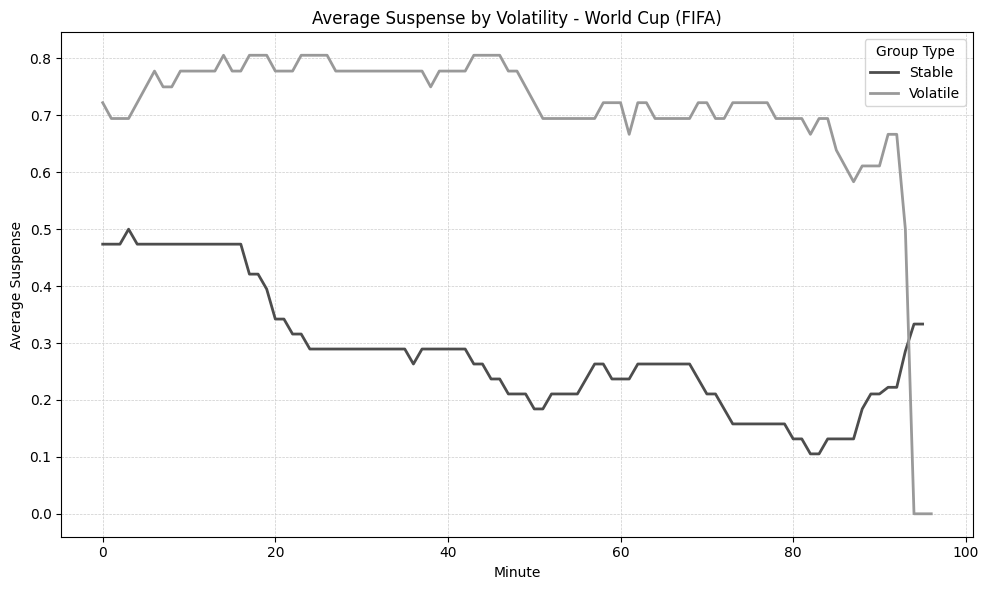
\includegraphics[width=1\textwidth]{images/susp_traj_wc_fifa.png}
    \caption{Suspense trajectories in World Cup groups (stable vs.\ volatile) under FIFA rules.}
    \label{fig:susp_traj_wc_fifa}
\end{figure}

\begin{figure}[H]
    \centering
    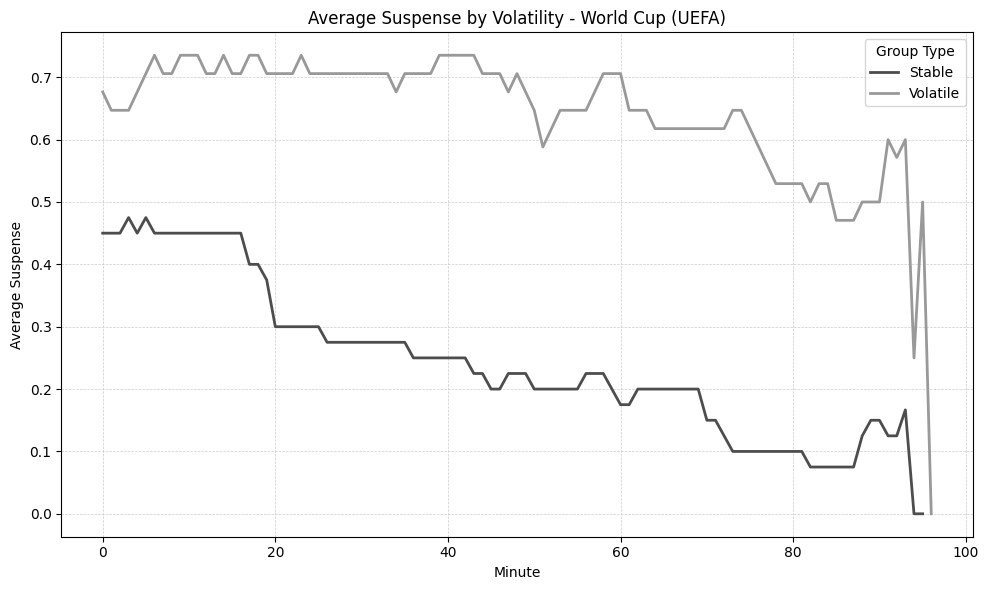
\includegraphics[width=1\textwidth]{images/susp_traj_wc_uefa.png}
    \caption{Suspense trajectories in World Cup groups (stable vs.\ volatile) under UEFA rules.}
    \label{fig:susp_traj_wc_uefa}
\end{figure}


\subsection{European Championship Suspense Trajectories}
\label{app:euro_trajectories}

Figures~\ref{fig:susp_traj_eu_uefa} and~\ref{fig:susp_traj_eu_fifa} display the suspense trajectories for stable and volatile groups in the European Championship under UEFA and FIFA rules respectively. Under UEFA's criteria (Figure~\ref{fig:susp_traj_eu_uefa}), the difference between the two trajectories is minimal at the start and end of matches, with the largest gap emerging between the 30th and 50th minutes. Under FIFA's criteria (Figure~\ref{fig:susp_traj_eu_fifa}), the gap starts at about 0.3 points and gradually narrows toward 0.2 points. In both cases, the differences are smaller in magnitude than those observed in the World Cup, consistent with the null result from the statistical tests and the regression estimation.

\begin{figure}[H]
    \centering
    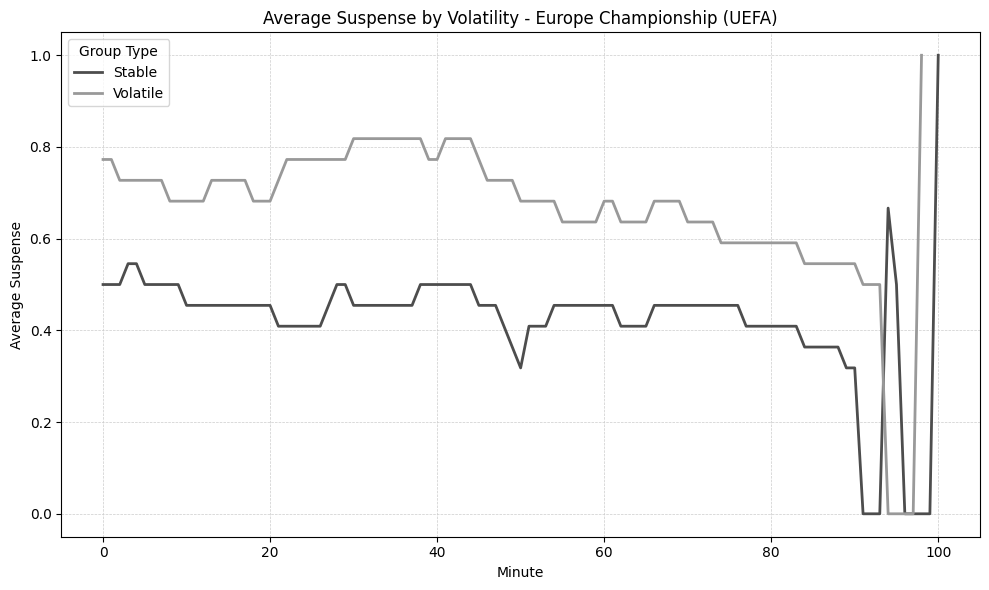
\includegraphics[width=1\textwidth]{images/susp_traj_eu_uefa.png}
    \caption{Suspense trajectories in European Championship groups (stable vs.\ volatile) under UEFA rules.}
    \label{fig:susp_traj_eu_uefa}
\end{figure}

\begin{figure}[H]
    \centering
    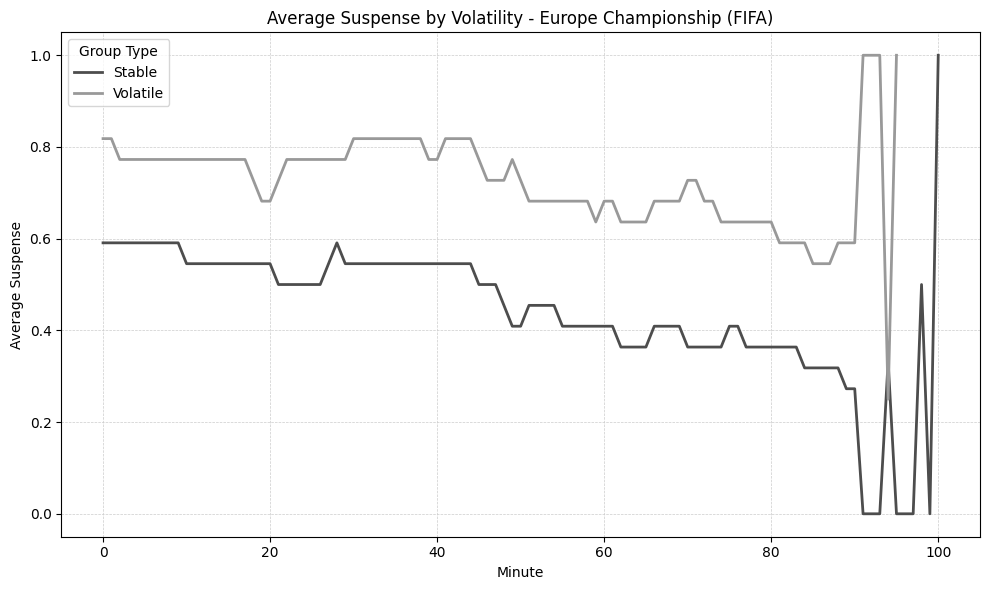
\includegraphics[width=1\textwidth]{images/susp_traj_eu_fifa.png}
    \caption{Suspense trajectories in European Championship groups (stable vs.\ volatile) under FIFA rules.}
    \label{fig:susp_traj_eu_fifa}
\end{figure}


\end{document}
